\documentclass[../main]{subfiles}
\ifSubfilesClassLoaded{
    \dominitoc
    \tableofcontentsfile
}{}
\begin{document}

\chapter{Analyse de l'auto-organisation de CxSOM}\label{chap:analyse}
\graphicspath{{06-Analyse/},{./}}
\minitoc

\section{Introduction}

Cette thèse s'inscrit dans une démarche expérimentale d'analyse d'un système complexe.
Nous avons proposé un modèle de connexions de cartes auto-organisatrices au sein d'une architecture complète.
Ce modèle s'appuie sur des modèles de connexions entre cartes existant dans la littérature, utilisés notamment dans le cadre des cartes récurrentes: la transmission de la position du BMU entre cartes.
La démarche expérimentale est constructive: nous proposons un modèle qui semble pertinent au regard des résultats existants dans la littératures. Nous cherchons ensuite à évaluer la pertinence du modèle et identifier des comportements.
Nous avons présenté ce modèle et les méthodes de représentations sur lesquelles nous nous appuierons.
L'expérience présentée en exemple du chapitre représentations a permis d'identifier quelques comportements élémentaires émergeant des connexions entre cartes.

A partir des comportements que nous observerons sur plusieurs ensembles de données, nous chercherons d'abord à définir comment s'effectue l'apprentissage multimodale dans une structure de cartes.
Une fois ces comportements définis, nous effectuerons une analyse paramétrique sur des petites architectures.
A l'issue de ce chapitre, nous serons donc en mesure de construire des architecture de 2 et 3 cartes et d'identifier leur capacité d'apprentissage. Nous concluerons sur la scalabilité du modèle à des architectures comportant un plus grand nombre de carte.

\subsection{Méthode expérimentale}

Nous réaliserons dans ce chapitre des expériences sur différentes structures de données d'entrées. Ces entrées sont tirées de modèles géométriques, nous permettant de définir des propriétés et de maîtriser les dépendances entre entrées.

Nous réutiliserons l'expérience présentée au chapitre représentation, sur des données disposée en cercle. Cette disposition est symétrique et laisse deux possibilités pour chaque entrée en sachant la première.
Nous faisons varier cette propriété en observant le comportement de deux cartes sur des entrées identiques (cas dégénéré), et sur des entrées indépendantes, prises aléatoirement. Entre ces deux cas dégénéré, nous observerons le comportement d'une architecture sur des exemples d'entrées différentes, dont les relations sont représentées en figure.
Nous choississons d'ajouter du bruit aux données: le cercle sera en fait un anneau, etc.

Nous élargissons également le jeu de données disponible à des entrées géométriques en trois dimensions. L'architecture de cartes utilisée sera alors une archiecture de trois cartes reliées réciproquement.
Ces entrées sont un cercle pivoté en trois dimensions, une surface quelconque, une sphere, et une repartition en volumes. Dans chacun de ces cas, le $U$ générant les entrées est de dimension différente: 1 pour une courbe,  2 pour une surface, 3 pour un volume.

Les architectures étudiées sont des architectures de cartes en une dimension. Nous choisissons d'identifier les comportements d'apprentissage sur des cartes en une dimension, facilement tracables, puis nous observerons si des cartes 2D présentent les mêmes comportements.

L'analyse paramétrique sera menée sur l'expérience du cercle. Nous avons en effet observé que le comportement des cartes selon différentes courbes est générique. Nous nous restreignons alors à étudier les paramètres du modèle sur un exemple particulier.

\begin{figure}
	\begin{minipage}{\textwidth}
		\begin{minipage}{0.33\textwidth}
			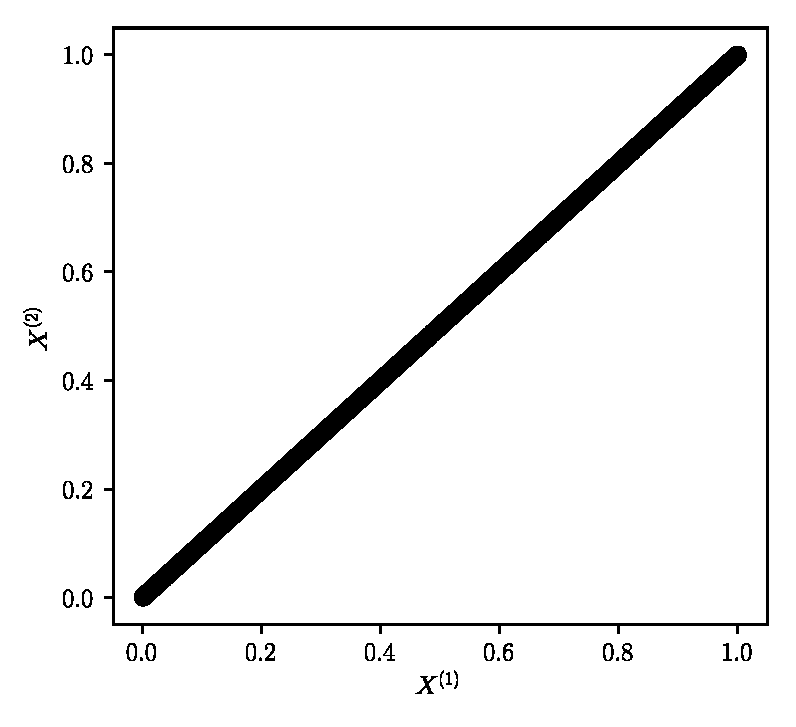
\includegraphics[width=\textwidth]{2som_id_in.pdf}
		\end{minipage}
		\begin{minipage}{0.33\textwidth}
			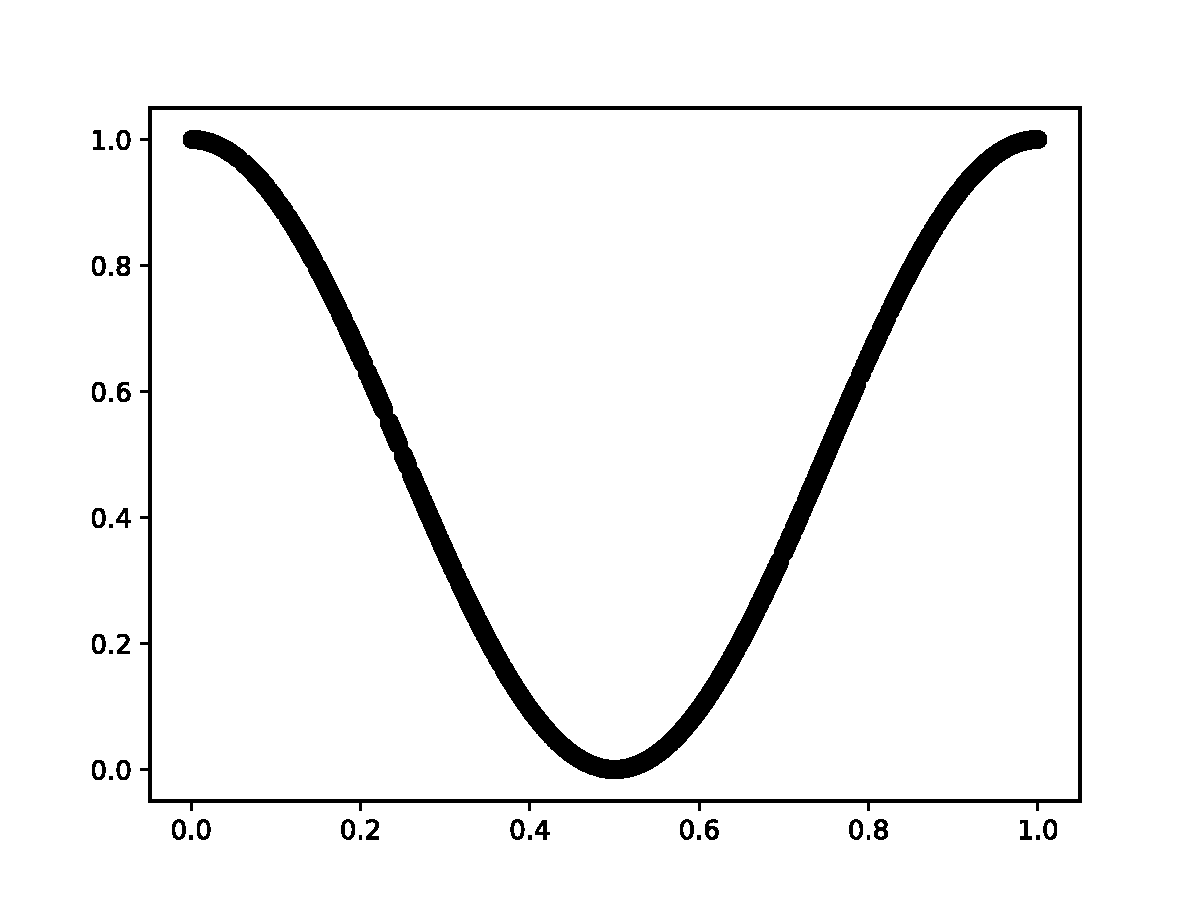
\includegraphics[width=\textwidth]{2som_courbe000_inputs.pdf}
		\end{minipage}
		\begin{minipage}{0.33\textwidth}
			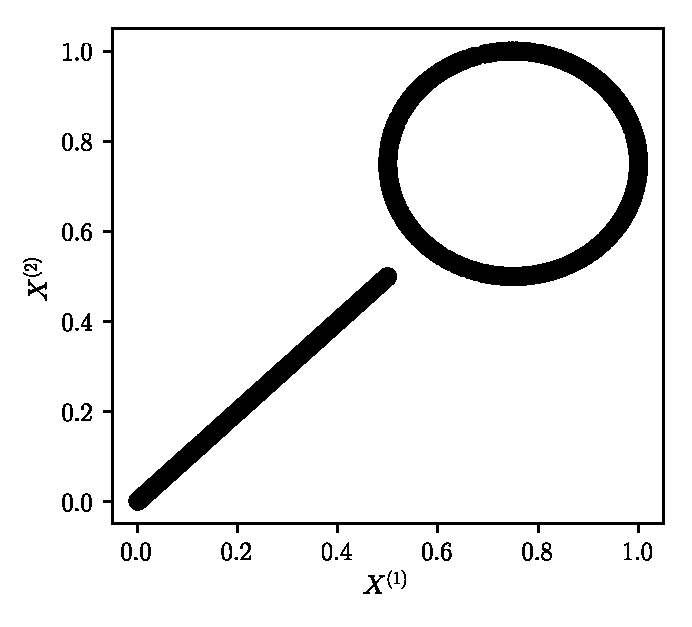
\includegraphics[width=\textwidth]{2som_mix_in.pdf}
		\end{minipage}
	\end{minipage}
	\begin{minipage}{\textwidth}
		\begin{minipage}{0.33\textwidth}
			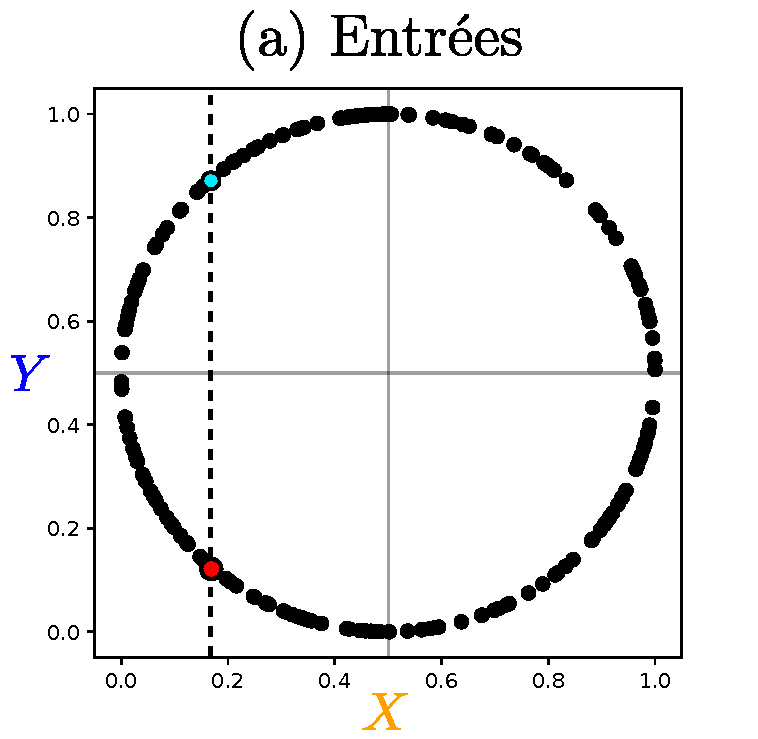
\includegraphics[width=\textwidth]{2som_inp_noU.pdf}
		\end{minipage}
		\begin{minipage}{0.33\textwidth}
			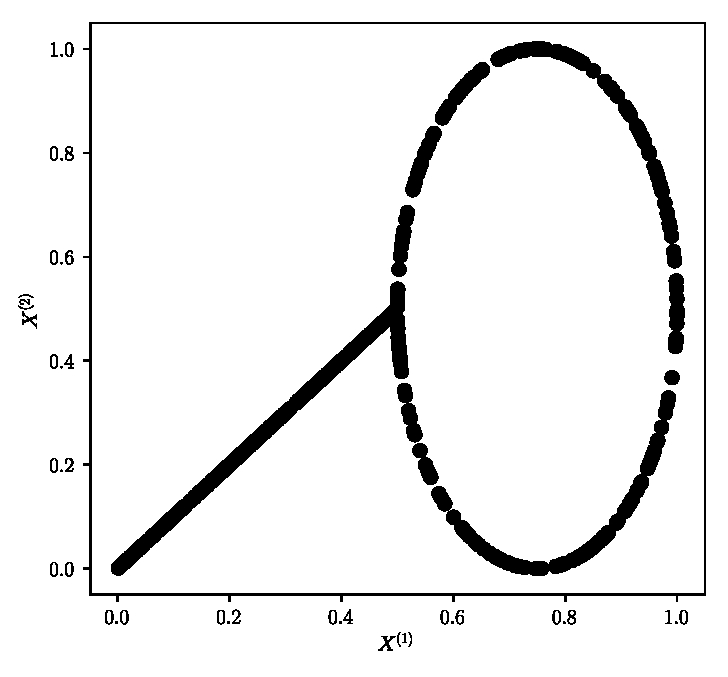
\includegraphics[width=\textwidth]{2som_mix001_in.pdf}
		\end{minipage}
		\begin{minipage}{0.33\textwidth}
			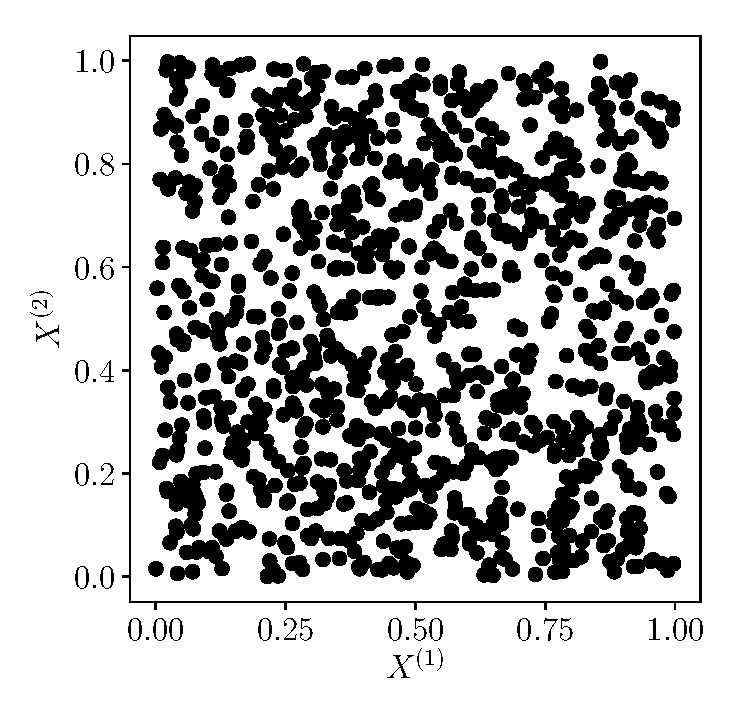
\includegraphics[width=\textwidth]{2som_square_in.pdf}
		\end{minipage}
	\end{minipage}
	
\end{figure}

\section{Quels comportements sont caratréristiques d'un apprentissage ?}
Dans ce chapitre, nous analyserons ces comportements plus en détail, et identifierons les comportements \emph{systémiques} émergeant d'une architecture simple à deux et trois cartes.

\subsection{Quantification vectorielle sur les entrées externes}

On veut d'abord que les poids externes de la carte encodent l'information de l'entrée. Ce sont en effet ces poids qui nous permettrons de faire de la prédiction ensuite.
Sur les différentes entrées, cette quantification est correctement réalisée. 
Cette quantification sur chaque carte est une première condition à vérifier pour évaluer l'organisation d'une architecture.

\subsection{Découpage d'une carte 1D et 2D en zones grâce aux poids contextuels}

Une architecture de cartes est un système complexe. 
Dans une logique de construction d'architecture, nous voulons d'abord identifier des comportements collectifs de cartes qui pourraient être intéressants dans l'apprentissage de données multimodales.
Nous avons choisi d'identifier ces comportements collectifs sur des petites architectures de deux et trois cartes en une dimension. Ces architectures sont représentables graphiquement.

Nous utiliserons la cartographie des entrées en fonction des BMUs dans deux dispositions d'entrées.
Dans toutes les dispositions, les modalités sont les coordonnées d'un point.
Nous considérerons des entrées tirées sur un cercle en deux et trois dimensions.
Dans cette disposition, chaque abcsisse $x$ correspond à deux valeurs de $y$, et inversement.
Dans cette disposition, nous ajoutons un bruit: le cercle sera en fait un anneau. Nous souhaitons ainsi évaluer si les cartes sont résistantes au bruit d'entrée et apprennent une représentation de la structure débruitée.
Nous étudierons également une disposition d'entrée prise sur l'ensemble du carré unité. Cette disposition d'entrée permet d'étudier comment une carte se comporte dans le cas ou il n'existe pas de relation entre les entrées.

Analysons d'abord la forme des poids contextuels de $M\m{1}$, que nous avions tracés en figure~\ref{fig:weights} sans les commenter. Les poids externes, en orange, présentent une disposition similaire à ceux observés dans la carte classique (b). Les poids contextuels, en bleu, présentent une forme de vagues, avec 7 valeurs de maximum allant de 0.5 à 1, et 6 minimum allant de 0.5 à 0.1. Ces maximum et minimum sont répartis en zones de taille équivalente sur la carte. 

Lorsqu'on s'intéresse au tracés des échantillons, on remarque d'abord que les positions dans la carte $M\m{1}$ se répartissent en zones étant BMUs et zones mortes, dans lesquelles aucune entrée n'a gagné. C'est une première différence avec la carte indépendante, pour laquelle toutes les positions gagneront pour des entrées. Les zones dans lesquelles il y a des BMUs correspondent aux extremum des poids contextuels et leurs alentours. C'est un phénomène inhabituel pour une carte de Kohonen. Les entrées $\inpx\m{1}$, dans la carte classique (b), correspondent à la courbe de poids externe: la valeur du poids du gagnant est toujours très proche de la valeur de l'entrée. Dans la carte $M\m{1}$, les entrées externes $\inpx\m{1}$ orange sont proches de la courbe de poids externes, mais avec plus d'erreur de quantification.
Les deux points rouge et bleu ayant la même valeur de $x$ ont un BMU différent dans la carte $M\m{1}$, alors que ces deux échantillons ont le même BMU dans la carte apprenant indépendamment sur les valeurs de $x$. Ainsi, la carte connectée au sein de CxSOM différencie les échantillons en fonction de non seulement leur entrée externe, mais aussi de l'entrée de l'autre carte de l'architecture. La plage de valeurs des $\inpx\m{1}$ gagnant dans un des zones recoupe les plages de valeurs gagnant dans les zones situées à gauche et à droite. Par exemple, la zone dans laquelle l'échantillon rouge gagne, autour de $\bmu\m{1} = 0.25$. La partie des entrées située en dessous de la courbe de poids externe recoupe les valeurs d'entrées gagnant dans la zone précédente; la partie située au dessous de la courbe de poids externe recoupe des valeurs gagnant dans la partie suivante. Pour une entrée externe, le choix de la zone de BMU dans laquelle elle gagnera dépend alors de l'entrée contextuelle. 


Dans la carte $M\m{1}$, une unité se spécialise donc par rapport aux deux entrées et non pas une seule comme dans la carte indépendante: les entrées externes et l'entrée contextuelles. C'est bien ce à quoi on s'attendait en ayant deux couches de poids. Ce qui est intéressant est que cette différenciation est réalisée par la répartition des unités en un nombre fini de zones distinctes. Dans chaque zone, les unités sont BMUs pour un segment de valeurs d'entrée externe et contextuelles. Au sein d'une zone, la répartition des entrées externe selon le BMUs est ordonnée, comme ce serait le cas dans une carte auto-organisatrice classique. Le comportement de la carte au sein d'une zone reste donc similaire à celui d'une carte classique.

Deux zones adjacentes correspondent par ailleurs à des segments de valeur d'entrée en partie superposés, et des segments de valeurs d'entrées contextuelles différentes. Il s'agit d'une deuxième échelle d'organisation, qui garde également l'aspect ordonné d'une carte classique. Ces zones sont créées par auto-organisation; aucun paramètre de la carte n'a été modifié pendant l'apprentissage pour former ces zones, et le nombre d'unités allouées par auto-organisation dans chaque zone est à peu près égal. La carte agit un peu comme une base de données structurée avec des indices primaires et des indices secondaires pour chaque neurone, l'indice primaire étant la zone de la carte, et l'indice secondaire la position dans cette zone.

\begin{figure}
	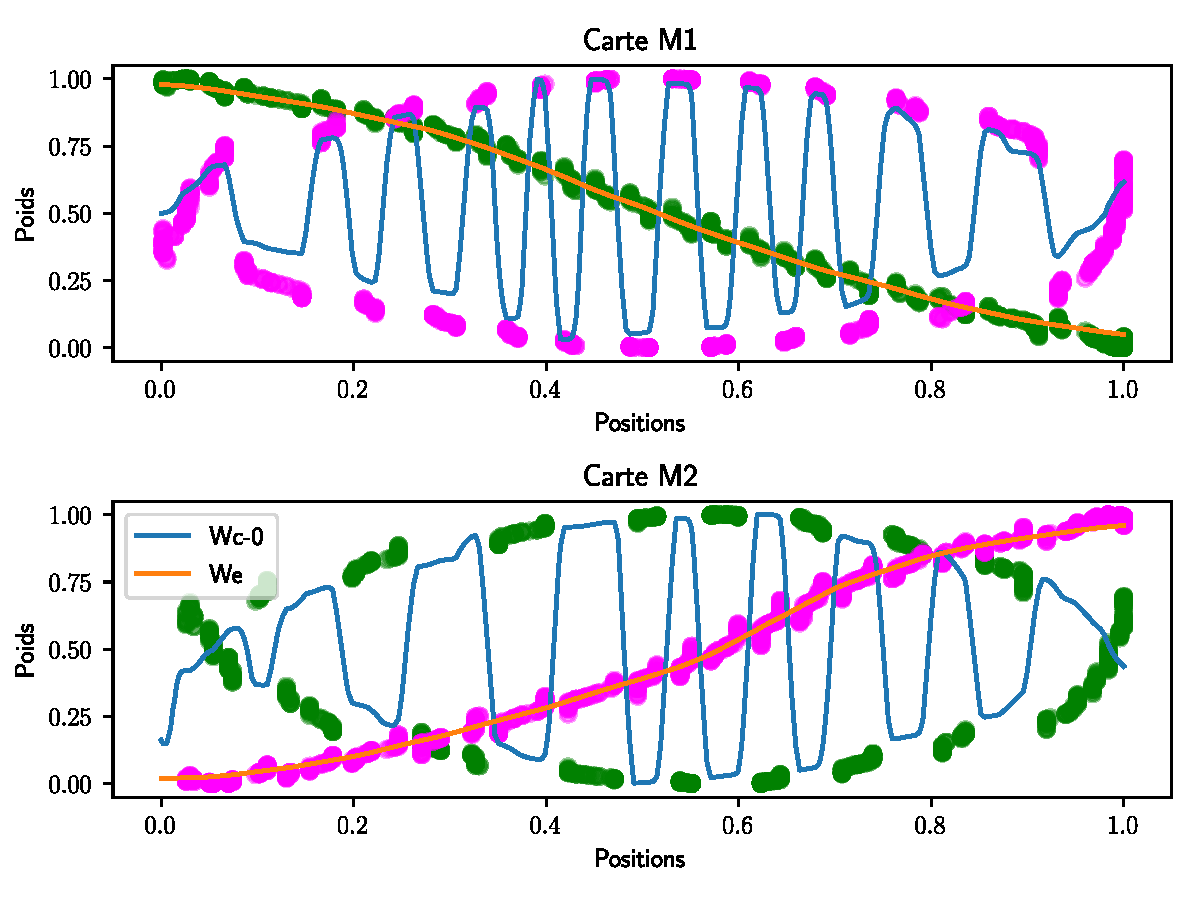
\includegraphics[width=0.7\textwidth]{2som_cercle_w.pdf}
\end{figure}

\begin{figure}
	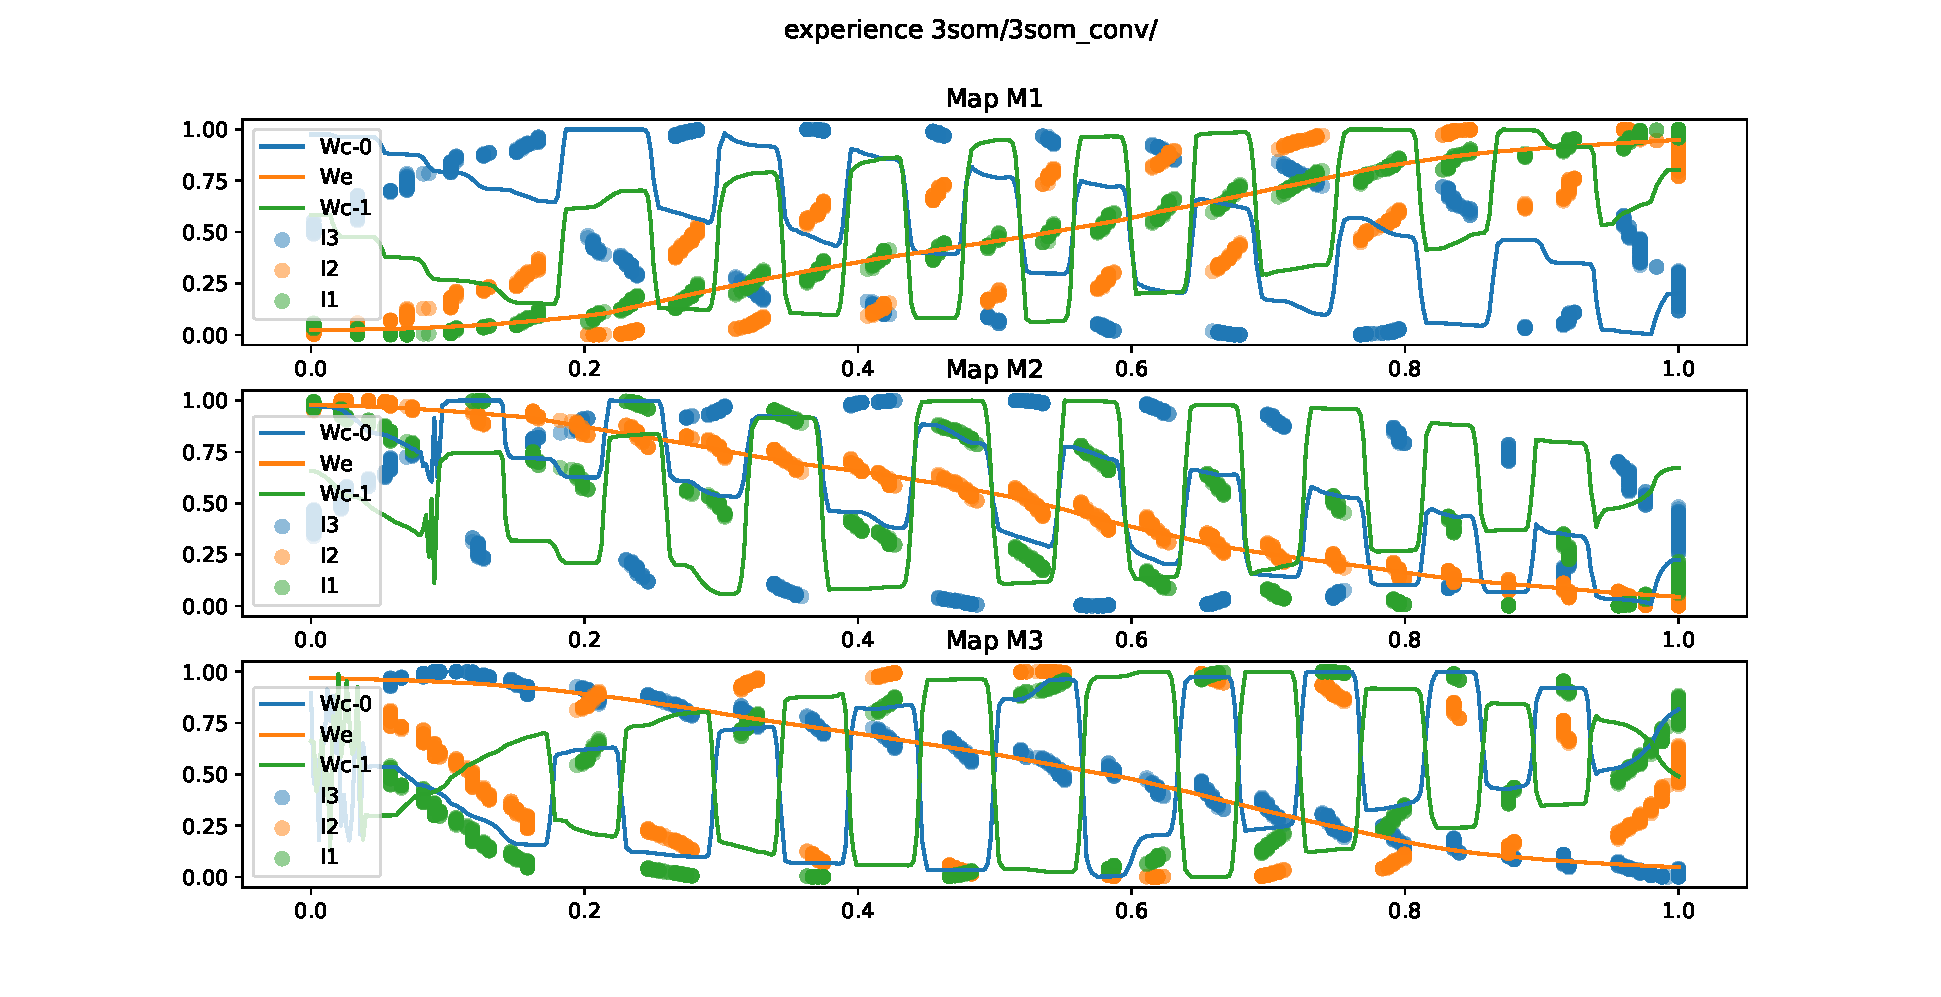
\includegraphics[width=0.7\textwidth]{3som_cercle_w.pdf}
\end{figure}

Cherchons à généraliser ce comportement: la disposition en zones traduit elle l'existence de l'apprentissage d'une relation entre entrée ?
Nous tracons la représentation cartographique des poids des deux cartes sur d'autres dispositions d'entrées: 
\begin{itemize}
	\item Lorsque $\inpx\m{1} = \inpx\m{2}$. La relation entre les deux entrées est alors une bijection. On s'attend à ce qu'on n'ai pas besoin de zones.
	\item Lorsque $\inpx\m{2} = 0.5+0.5*\cos(2*\pi*\inpx\m{1})$. La relation entre les deux entrées est une fonction. On s'attend à ce que $M\m{2}$ présente des zones, car une même valeur de $\inpx\m{2}$ correspond à plusieurs valeurs de $\inpx\m{1}$, mais que $M\m{1}$ ne s'organise pas en zones.
\end{itemize}

\begin{figure}
\begin{minipage}{0.66\textwidth}
	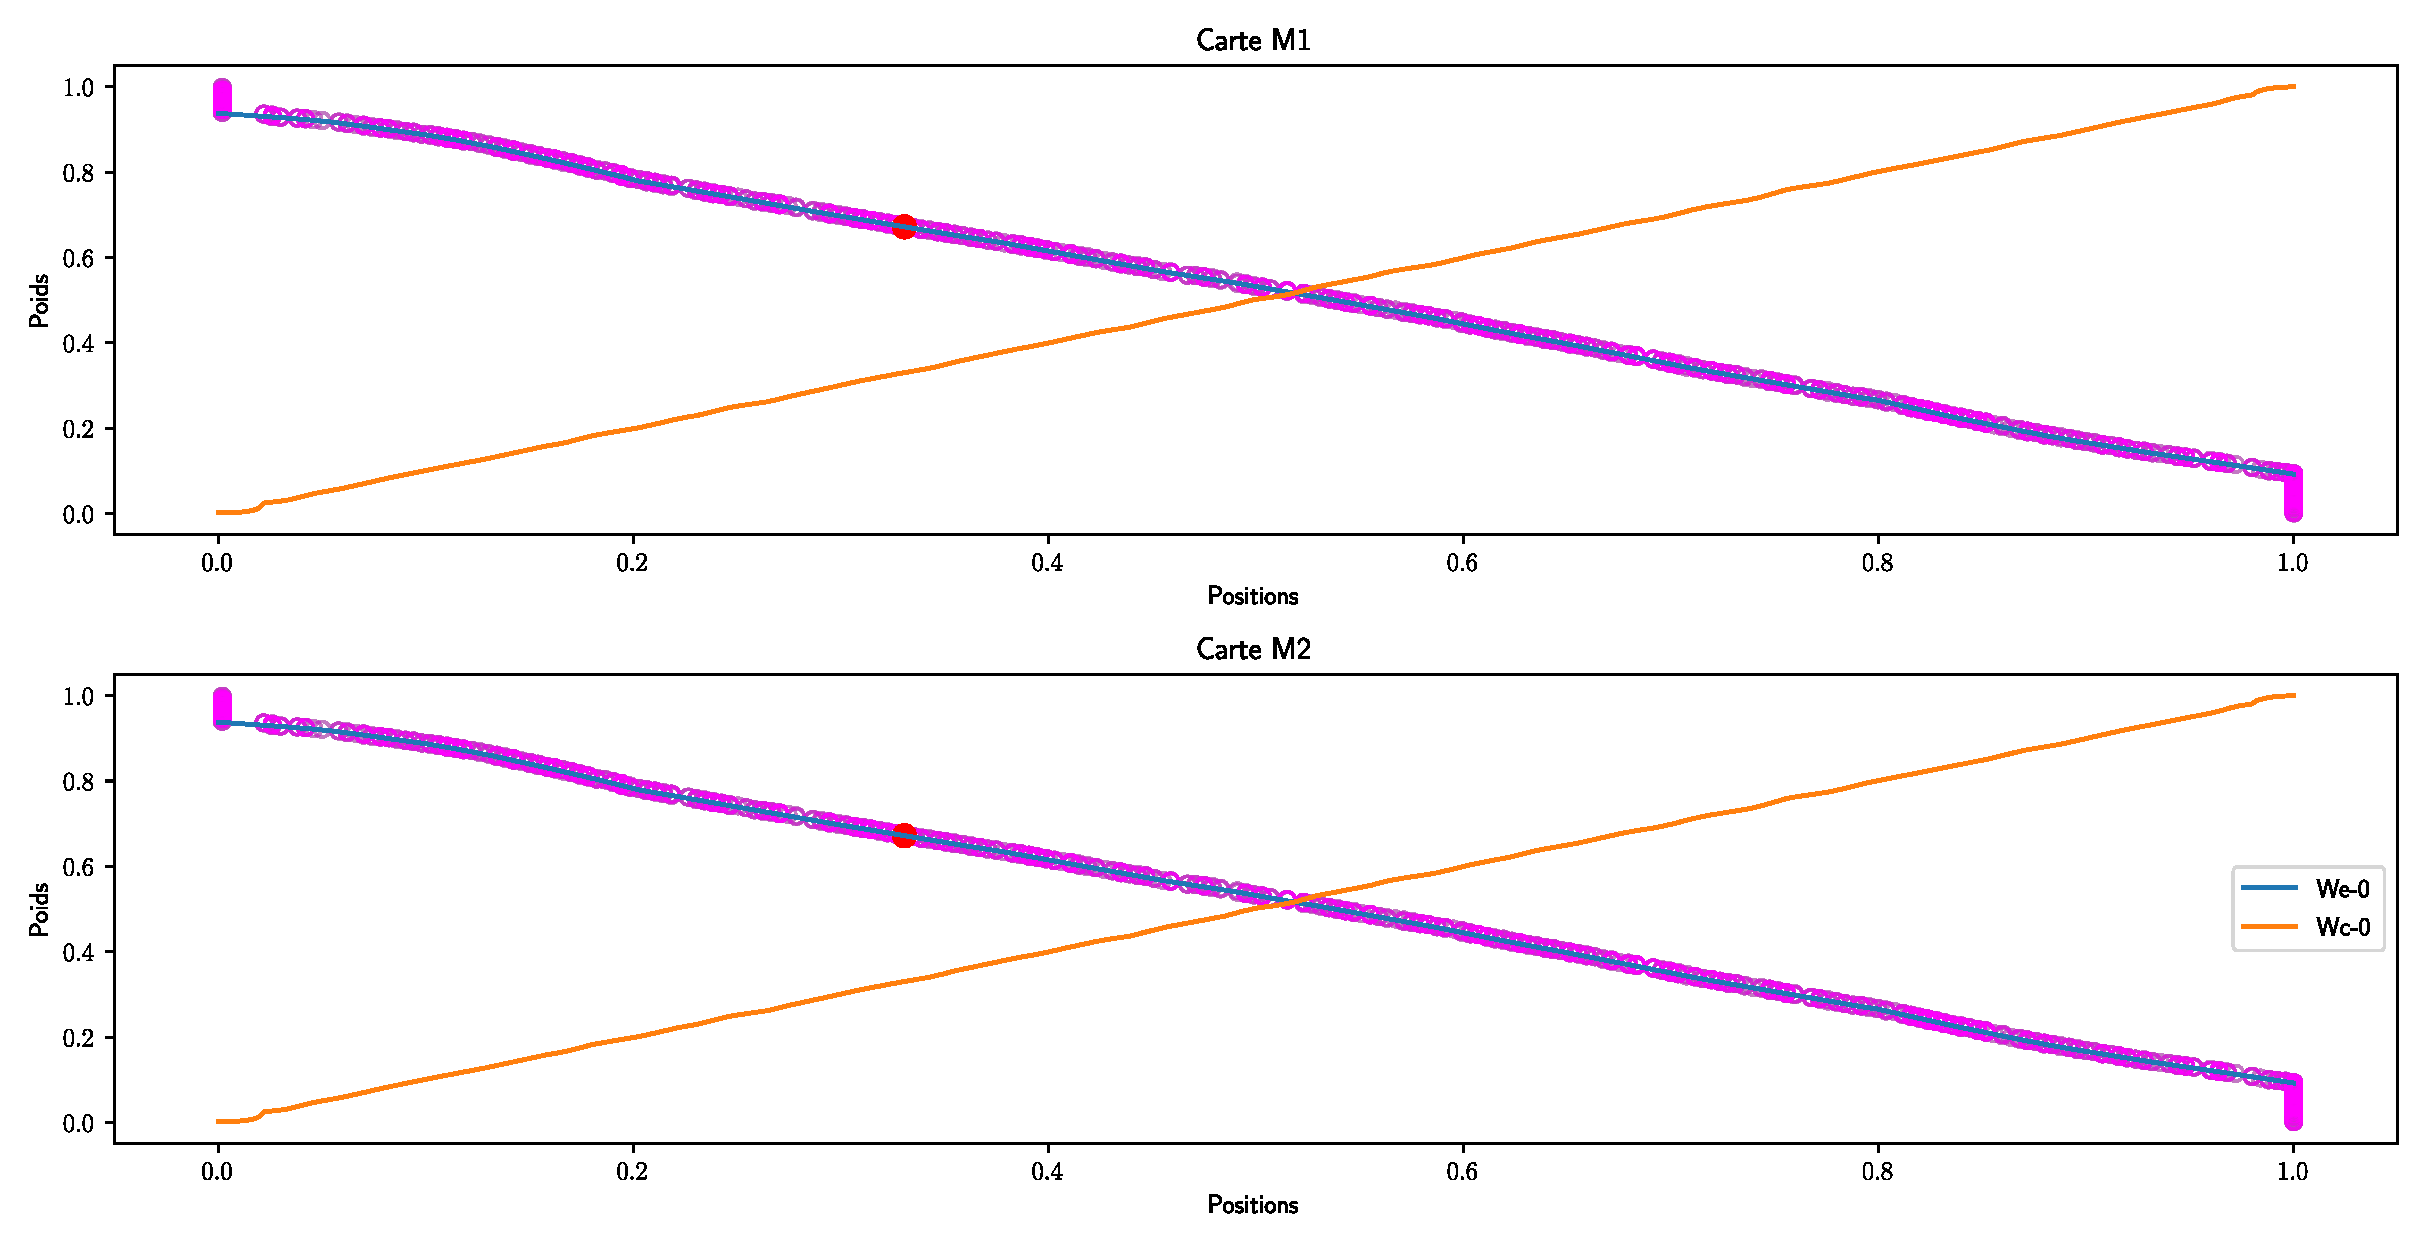
\includegraphics[width=\textwidth]{2som_id_w.pdf}
	\caption{Représentation cartographique des poids et entrées pour la disposition identité}
\end{minipage}
\begin{minipage}{0.33\textwidth}
	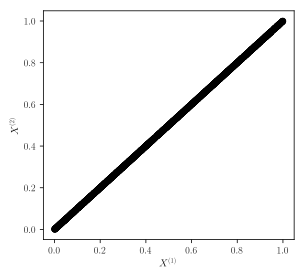
\includegraphics[width=\textwidth]{2som_id_in}
\end{minipage}
\end{figure}

\begin{figure}
	\begin{minipage}{0.66\textwidth}
	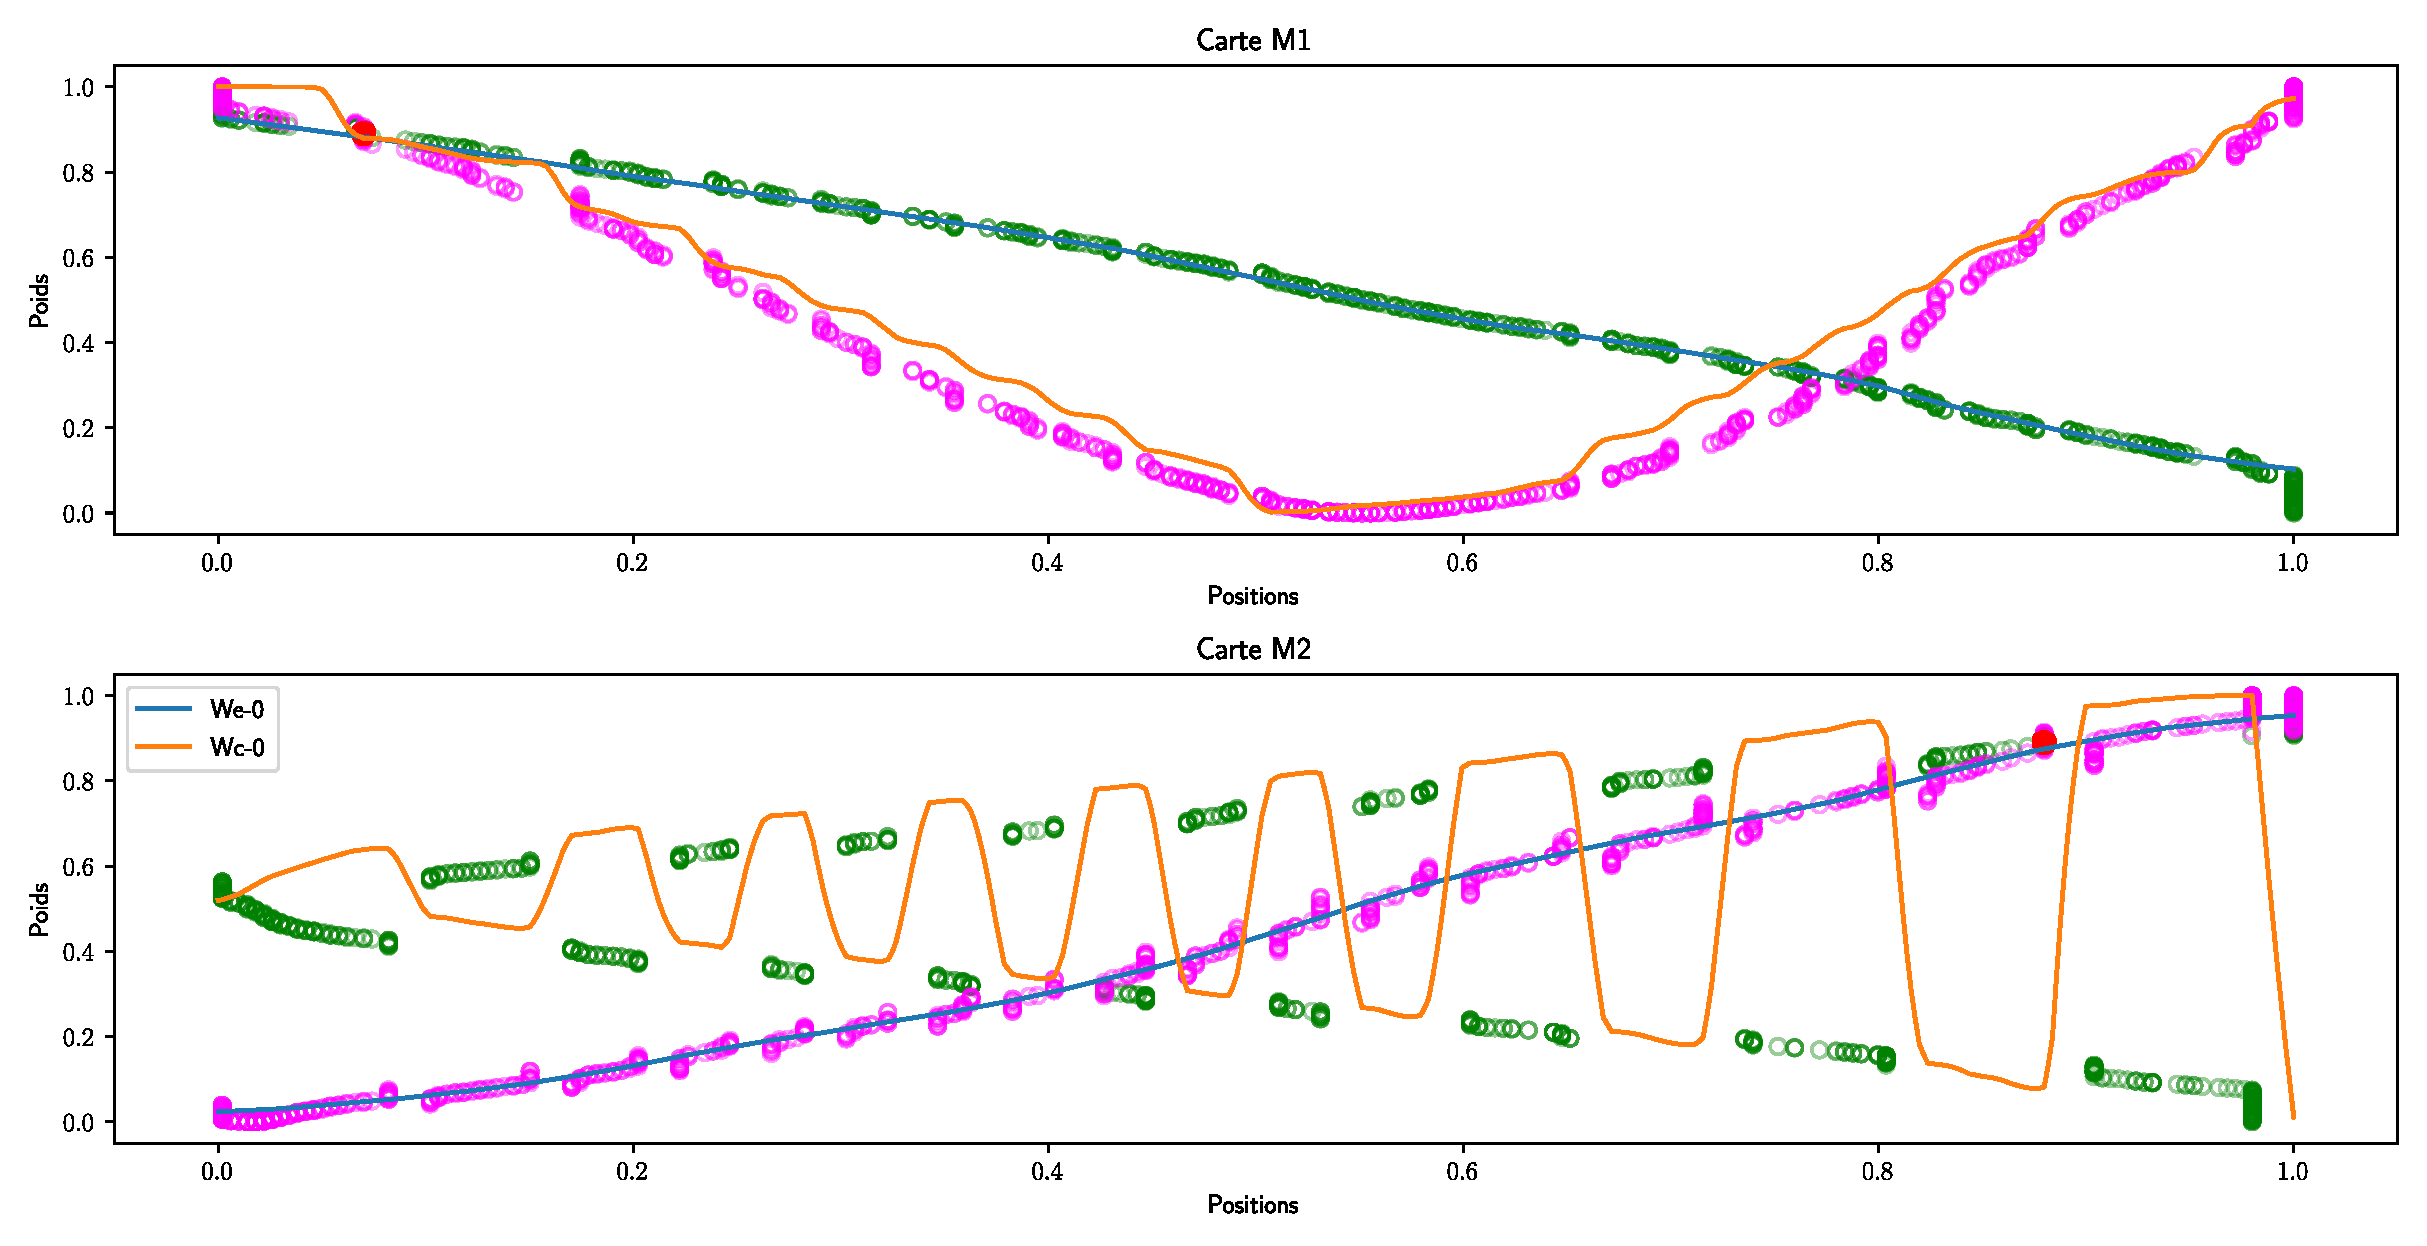
\includegraphics[width=\textwidth]{2som_cos_w.pdf}
	\caption{Représentation cartographique des poids et entrées pour la disposition cos}
	\end{minipage}
	\begin{minipage}{0.33\textwidth}
		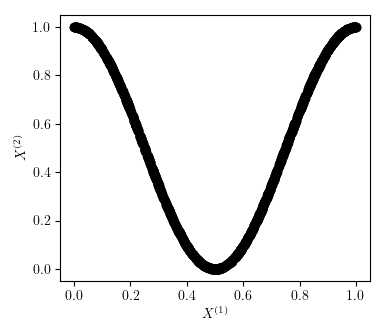
\includegraphics[width=\textwidth]{2som_cos_in.png}
	\end{minipage}
\end{figure}

\begin{figure}
	\begin{minipage}{0.66\textwidth}
		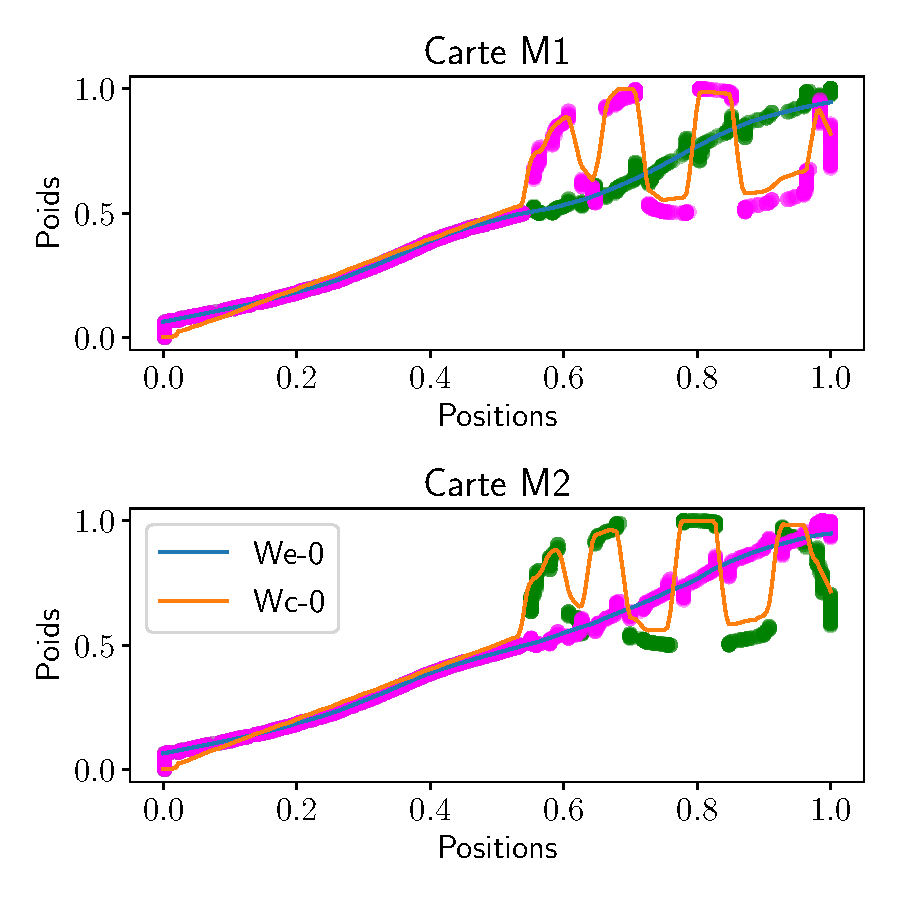
\includegraphics[width=\textwidth]{2som_mix_w.pdf}
	\caption{Représentation cartographique des poids et entrées pour la disposition mix}
	\end{minipage}
	\begin{minipage}{0.33\textwidth}
		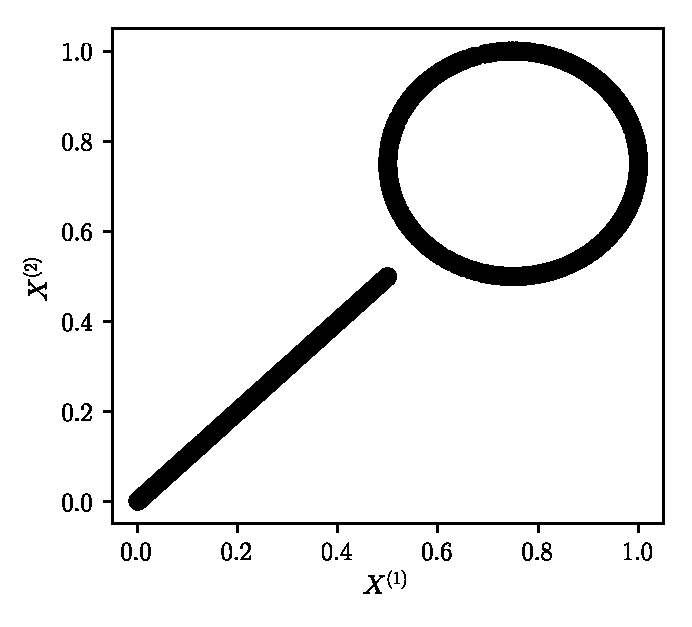
\includegraphics[width=\textwidth]{2som_mix_in.pdf}
	\end{minipage}
\end{figure}

\begin{figure}
	\begin{minipage}{0.66\textwidth}
		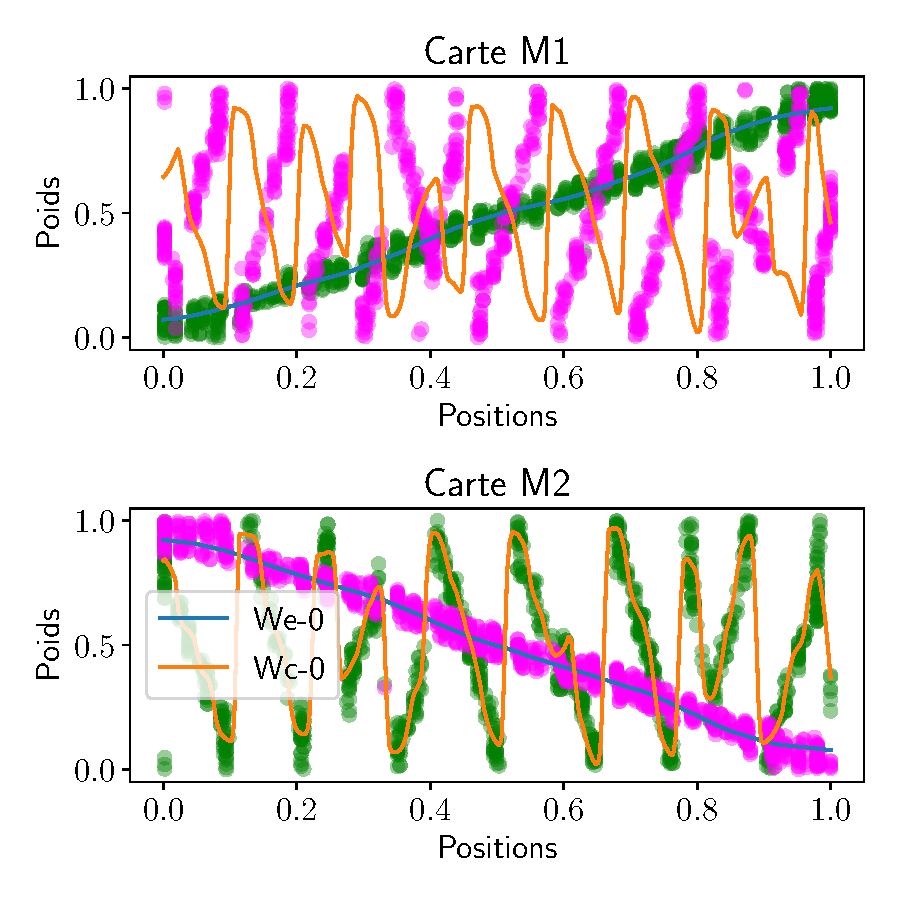
\includegraphics[width=\textwidth]{2som_square_w.pdf}
	\caption{Représentation cartographique des poids et entrées pour la disposition mix}
	\end{minipage}
	\begin{minipage}{0.33\textwidth}
		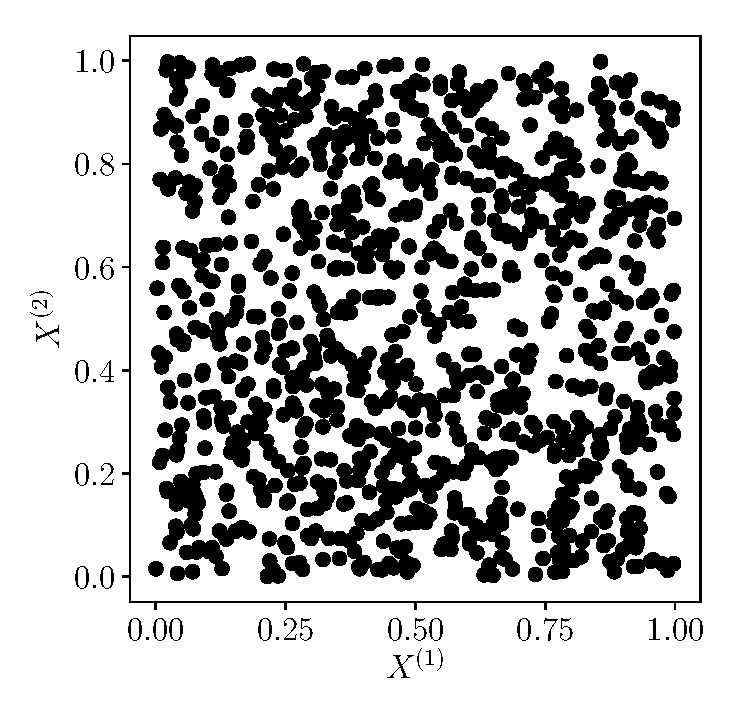
\includegraphics[width=\textwidth]{2som_square_in.pdf}
	\end{minipage}
\end{figure}


\begin{itemize}
	\item Organisation en zones dès que besoin de découpler deux valeurs de U
	\item Le comportement traduit l'existence de plusieurs valeurs de U pour une même entrée, sans forcément qu'une relation existe. Dans tous les cas, la carte effectue un découpage selon U.
	\item Lorsque relation il y a, ce découpage permet de faire de la prédiction.
\end{itemize}

\subsection{Différenciation de $U$ selon les BMUs: indicateur d'une mémoire associative}



\subsection{Qu'appelle t'on apprentissage des données multimodales ?}

A partir des comportements observés, définissons les comportements marquant l'apprentissage de données multimodales, et quelles mesures indiquent l'existence de cet apprentissage.
Le but de la mémoire assoctative est d'apprendre des données de plusieurs modalités et d'apprendre leurs associations. L'apprentissage des données indépendantes est donc un comportement nécessaire à cette mémoire associative. 
Nous avons observé sur les différentes expériences que le poids du BMU $\omega_e(\bmu)$ est proche de la valeur de l'entrée pour tout l'espace. La quantification vectorielle effectuée dans chaque carte est donc bonne, marquant l'apprentissage des données de façon indépendante. Nous aurons besoin de vérifier ce comportement comme indicateur du bon fonctionnement d'une architecture.

Le but de la mémoire associative est d'apprendre des relations entre les entrées. Comme une carte cherche à extraire une structure dans les données de son espace d'entrée, observe t-on l'apprentissage d'une structure dans les relations entre entrées dans l'architecture de cartes ? 
Cet apprentissage de relations passe par la disposition en zones auto-organisées au sein d'une carte. Ces zones, nous l'avons vu, déterminent la BMU de chaque carte en fonction de l'ensemble des entrées et non seulement de l'entrée de la carte en question. Ces zones ne marquent pas l'apprentissage d'une relation: dans les cas ou les entrées sont indépendantes, la carte se divise quand même en zones distinctes. La présence de zones est spécifique au comportement de l'architecture CxSOM.
L'apprentissa

\section{Prédiction d'entrée comme marqueur de la mémoire associative}


\subsection{Conclusion}

Ces architectures de quelques cartes sont des architectures \emph{élémentaires}: toute architecture comportant plus de cartes pourra être construite à partir de petits modules. Nous considérerons les comportements observés dans ce chapitre comme des comportements élémentaires des architectures de cartes.

\section{Etude des paramètres}
Nous avons identifié les comportements générés dans CxSOM qui montrent un apprentissage des données multimodales. Nous comparerons dans cette section ces comportements pour différents paramètres pour une architecture de trois cartes.


\section{Extension sur deux dimensions}

maj du 5 juillet:
2som2D in4D simulée, et code pour les affichage faits.

Les comportements d'une architecture de carte ont été mis en lumière sur des cartes 1D et des entrées 1D. Nous présentons dans cette section les comportements observés sur une architecture de deux cartes de type grille en deux dimensions. 
Nous travaillons à présent sur des entrées en deux dimensions. Ces entrées sont les coordonnées 4D d'une sphere 3D dont on a effectuée une rotation dans l'espace en 4D, de la même façon que les entrées en 3D se trouvaient sur un cercle 2D dont on a effectué une rotation dans l'espace.
Nous prenons une architecture de deux cartes, prenant chacune une paire d'entrées $X,Y$ et $Z,T$. Les entrées ayant un rôle symétrique, la paire choisie importe peu.
Nous attendons de retrouver les comportements des cartes en une dimension sur les cartes en deux dimensions. Les entrées considérées étant similaires aux expériences précédentes, on devrait retrouver les comportements.

Ces cartes apprennent sur une sphere qui est "tournée" dans l'espace 4D, Ainsi, si on trace n'importe quel groupe de 3 coordonnée, ca fait un truc sphérique. Chaque carte prend deux coordonnées.
On a un U en 2 dimensions (coordonnées polaires d'une sphere)
Voici les vidéos des tracés des poids externes et contextuels (2D) de chaque carte.
Voici le tracé des erreurs de quantification dans chaque carte, ainsi que uv.
Il semble que bien qu'on retrouve le comportement en sous indices, on n'apprend pas spécialement de relations sur des cartes 2D. Selon moi, il faudrait d'explorer un grand nombre de paramètres pour éventuellement trouver un comportement émergeant. L'existence d'un tel comportement n'est pas exclu mais rien ne le garantit.



\ifSubfilesClassLoaded{
    \printbibliography
    %\externaldocument{../main.tex}   
}{}
\end{document}